\section{CoarseGrainedTree}
\label{coarsegrainedtree}


\begin{figure}[H]
	\centering
	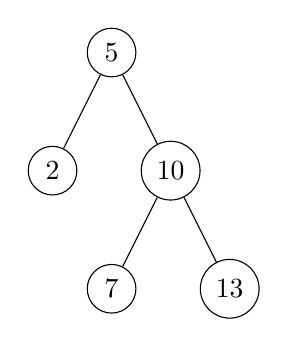
\begin{tikzpicture}
	    \tikzstyle{every node}=[circle,draw]
	    \node {5}
	        child { node {2} }
	        child {
	            node {10}
	            child { node {7} }
	            child { node {13} }
	        }
	    ;
	\end{tikzpicture}
	\caption{Example of binary search tree}
	\label{fig:tree}
\end{figure}

A Binary Search Tree (BST) is another basic structure as the list. It is represented with nodes and leafs. Each node is composed by a value and two pointers which link to its subtrees.


Considering the value of a generic node as V, every node on its right subtree contains a value greater than V, and on its left subtree all the values are lesser or equal at V. \newline


The insertion of a new element in the tree starts from the root and goes to the right or left subtree according to the value of the current node, until reaching the leaf. When a new element is already present in the tree, its is added as a new left child node of the first occurrence of the equal element. If the node already have a left child this will become the left child of the new node.


Removing an element from the tree consist of removing the first occurrence of the element and it will be replaced with one of the two children subtree.\newline


The \emph{toString} method will produce the following output for the tree represented in figure \ref{fig:tree}:\newline

\begin{lstlisting}
	[5[2][10[7][13]]]
\end{lstlisting}

According to the requirements, all the tree must be locked during the updating procedures so it will need only one lock for the whole structure. As in the CoarseGrainedList, we can use the simple java Lock.

Unfortunately, using only one lock the structure is not scalable and with multiple threads only one  can work on it at time. This means that as well as the previous structure, there is no gain in performance with multiple threads.


The performance of the tree for a generic update is $\mathcal{O}(\log N)$, where $N$ is the number of nodes and $\log N$ is the depth of the tree.\newline

The structure of node can be represented as following:\newline

\begin{lstlisting}
	class Node<T>{
		T value;
		Node<T> left;
		Node<T> right;
	}
\end{lstlisting}

